\documentclass{article}
\usepackage{amsmath}
\usepackage{xcolor}
\usepackage{gensymb}
\usepackage{ragged2e}
\usepackage{graphicx}
\usepackage{gensymb}
\usepackage{mathtools}
\newcommand{\mydet}[1]{\ensuremath{\begin{vmatrix}#1\end{vmatrix}}}
\providecommand{\brak}[1]{\ensuremath{\left(#1\right)}}
\providecommand{\norm}[1]{\left\lVert#1\right\rVert}
\newcommand{\solution}{\noindent \textbf{Solution: }}
\newcommand{\myvec}[1]{\ensuremath{\begin{pmatrix}#1\end{pmatrix}}}
\let\vec\mathbf
\begin{document}
\begin{center}
        \textbf\large{CHAPTER-9 \\ AREAS OF PARALLELOGRAMS AND TRIANGLES}
\end{center}
\section{Exercise 9.2}
Q1. In the figure given below, $ABCD$ is a parallelogram, $AE \perp DC$ and $CF \perp AD$.If $AB = 16cm$, $AE = 8cm$ and $CF = 10cm$, find $AD$.\\
\textbf{Construction}
\begin{figure}[h]
 \begin{center}
  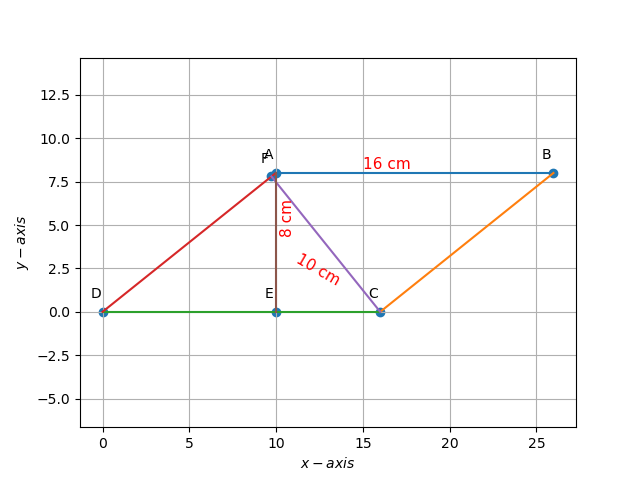
\includegraphics[width=\columnwidth]{fig1.png}
 \end{center}
 \caption{Parallelogram ABCD}
 \label{fig:Fig1}
\end{figure}\\
The following table displays the given input parameters :\\
\begin{table}[h]
	\centering
	\begin{tabular}{|c|c|c|}
\hline
Symbol & Value & Description\\
\hline
$a$ & 10cm & CF \\
\hline
$b$ & 8cm & AE \\
\hline
$l$ & 16cm & AB \\
\hline
$\angle{AED}$ & $90\degree$ & AE $\perp$ DC \\
\hline
$\angle{DFC}$ & $90\degree$ & CF $\perp$ AD \\
\hline
\end{tabular}

	\caption{Input Parameters}
	\label{tab:table1}
\end{table}\\
The lengths and angles which are to be found out are displayed in the table below along with their symbols :\\
\begin{table}[h]
	\centering
	\begin{tabular}{|c|c|}
\hline
Symbol & Description \\
\hline
$c$ & CD \\
\hline
$d$ & DE \\
\hline
$r$ & AD \\
\hline
$f$ & DF \\
\hline
$\theta$ & $\angle{D}$\\
\hline
\end{tabular}

	\caption{Unknown Parameters}
	\label{tab:table2}
\end{table}\\
The input co-ordinates of the above parallelogram is $\vec{D}$ which is at the origin.The rest of the point co-ordinates can be derived based on this assumption in the following way which is shown in the table below :\\
\begin{table}[h]
	\centering
	\begin{tabular}{|c|c|}
\hline
Point & Co-ordinates\\
\hline
$\vec{A}$ & $r\myvec{\cos{\theta}\\\sin{\theta}}$ \\
\hline
$\vec{B}$ & $\vec{A} + \vec{C}$ \\
\hline
$\vec{C}$ & $c\vec{e_1}$\\
\hline
$\vec{E}$ & $d\vec{e_1}$ \\
\hline
$\vec{F}$ & $f\myvec{\cos{\theta}\\\sin{\theta}}$ \\
\hline
\end{tabular}

	\caption{Unknown Co-ordinates}
	\label{tab:table3}
\end{table}\\
\textbf{Deriving the Unknown lengths and angles in terms of known and derived parameters :}\\
\begin{enumerate}
	\item \textbf{Deriving c:}
		From Figure\ref{fig:Fig1}, $c$ is  parallel to $l$(AB paralle to CD).So,
		\begin{align}
			c = l
			\label{eq:1}
		\end{align}
	\item \textbf{Deriving d:}
		From $\triangle{ADE}$,
		\begin{align}
			\cos{\theta} = \frac{DE}{AD} = \frac{d}{r}
			\implies d = r\cos{\theta}
			\label{eq:2}
		\end{align}
	\item \textbf{Deriving r:}
		From $\triangle{ADE}$,
		\begin{align}
			\sin{\theta} = \frac{AE}{AD} = \frac{b}{r}
			\implies r = \frac{b}{\sin{\theta}}
			\label{eq:3}
		\end{align}
	\item \textbf{Deriving f:}
		From $\triangle{DFC}$,
		\begin{align}
			\cos{\theta} = \frac{DF}{DC} = \frac{f}{c}
			\implies f = c\cos{\theta}
			\label{eq:4}
		\end{align}
	\item \textbf{Finding $\theta$:}
		From $\triangle{DFC}$,
		\begin{align}
			\sin{\theta} = \frac{CF}{CD} = \frac{a}{c}
			\implies \theta = \sin^{-1}\frac{a}{c}
			\label{eq:6}
		\end{align}
\end{enumerate}
From eq\ref{eq:1},eq\ref{eq:2},eq\ref{eq:3},eq\ref{eq:4} and eq\ref{eq:6}, table\ref{tab:table2} can be modified as :\\
\begin{table}[h]
	\centering
	\begin{tabular}{|c|c|c|}
\hline
Symbol & value & Description\\
\hline
$c$ & $l$ & DC\\
\hline
$r$ & $\frac{b}{\sin{\theta}}$ & AD \\
\hline
$d$ & $r\cos{\theta}$ & DE \\
\hline
$\theta$ & $\sin^{-1}\frac{a}{c}$ & $\angle{D}$ \\
\hline
$f$ & $c\cos{\theta}$ & DF\\
\hline
\end{tabular}


	\caption{Unknown parameters in terms of known and derived parameters}
	\label{tab:table4}
\end{table}\\
\textbf{Finding out unknown lengths and angles :}\\
\begin{enumerate}
	\item \textbf{Finding $\theta$:}
		From eq\ref{eq:6},
		\begin{align}
			\theta = \sin^{-1}\frac{10}{16} = 38.68\degree
			\label{eq:7}
		\end{align}
	\item \textbf{Finding c:}
		From eq\ref{eq:1},
		\begin{align}
			c = 16cm
			\label{eq:8}
		\end{align}
	\item \textbf{Finding r:}
		From \ref{eq:3}, the value of $r$ is :
		\begin{align}
			r = \frac{8}{\sin{38.68}} = 12.8cm
			\label{eq:9}
		\end{align}
	\item \textbf{Finding d:}
		From eq\ref{eq:2},
		\begin{align}
			d = (12.8)\cos{38.68} = 10cm
			\label{eq:10}
		\end{align}
	\item \textbf{Finding f:}
		From eq\ref{eq:4},
		\begin{align}
			f = (16)\cos{38.68} = 12.48cm
			\label{eq:11}
		\end{align}
\end{enumerate}
\textbf{Deriving co-ordinates in terms of known and derived parameters:}\\
Based on table\ref{tab:table4}, table\ref{tab:table3} can be modified as follows :\\
\begin{table}[h]
	\centering
	\begin{tabular}{|c|c|c|}
\hline
Point & Co-ordinates\\
\hline
$\vec{A}$ & $\frac{b}{\sin{\theta}}\myvec{\cos{\theta}\\\sin{\theta}}$\\
\hline
$\vec{B}$ & $\vec{A} + \vec{C}$\\
\hline
$\vec{C}$ & $c\vec{e_1}$\\
\hline
$\vec{E}$ & $r\cos{\theta}\vec{e_1}$\\
\hline
$\vec{F}$ & $c\cos{\theta}\myvec{\cos{\theta}\\\sin{\theta}}$\\
\hline
\end{tabular}

	\caption{Co-ordinates in terms of known and derived co-ordinates}
	\label{tab:table5}
\end{table}\\
Based on eq\ref{eq:7},eq\ref{eq:8},eq\ref{eq:9},eq\ref{eq:10} and eq\ref{eq:11} and table\ref{tab:table5}.The final co-ordinates of the  parallelogram are displayed in the table below:\\
\begin{table}[h]
	\centering
	\begin{tabular}{|c|c|}
\hline
Point & Co-ordinates\\
\hline
$\vec{A}$ & $\myvec{10\\8}$\\
\hline
$\vec{B}$ & $\myvec{26\\8}$\\
\hline
$\vec{C}$ & $\myvec{16\\0}$\\
\hline
$\vec{D}$ & $\myvec{0\\0}$\\
\hline
$\vec{E}$ & $\myvec{10\\0}$\\
\hline
$\vec{F}$ & $\myvec{9.75\\7.8}$\\
\hline
\end{tabular}

	\caption{Final Co-ordinates}
	\label{tab:table6}
\end{table}\\
From eq\ref{eq:9}, we got the length of AD = r = 12.8cm.
\end{document}
